\subsection{Evolución diferencial: Conceptos básicos}

Esta sección está dedicada a revisar la variante clásica de \DE{} y a introducir varios términos importantes que son utilizados 
en el campo de \DE{}.
%
El esquema clásico de \DE{} es identificado como \DE{}/rand/1/bin y ha sido ampliamente usado como base para el desarrollo de 
variantes más complejas~\cite{das2011differential}.
%
De hecho, la propuesta que se presenta en este capítulo como ejemplo extiende al \DE{}/rand/1/bin.
%
\DE{} fue propuesta como un método de búsqueda directo para optimización continuo mono-objetivo y es el ámbito en que
se usará en este capítulo, es decir, se considera la Ecuación~\ref{eqn:Model_general}, fijando $M = 1$.

\DE{} es un algoritmo estocástico basado en población, por lo que en cada instante maneja un conjunto de soluciones 
candidatas que van evolucionando de forma iterativa.
%
En \DE{} dichas soluciones candidatas son usualmente conocidas como vectores.
%
En la variante básica de \DE{}, para cada miembro de la población (conocido como \textit{vectores objetivo}) 
se genera un nuevo vector que es conocido como el \textit{vector mutado}.
%
A continuación, el vector mutado se combina con el vector objetivo para generar al \textit{vector de prueba} y 
finalmente se procede con la fase de selección para seleccionar a los vectores sobrevivientes.
%
De esta forma, las generaciones transcurren de forma iterativa hasta cumplir el criterio de paro.
%
En esta capítulo, el $i$-ésimo vector de la población en la generación $G$ se denota como$\vec{X}_{i,G} = [x_{1,i,G}, x_{2,i,G},..., X_{D,i, G}]$.
%
A continuación se explica en más detalle cada componente de \DE{}.

\subsubsection{Inicialización}

Usualmente, \DE{} inicia el proceso de optimización con una población de $NP$ vectores que son creados de forma aleatoria.
%
Habitualmente los vectores de la población inicial son generados en base a una distribución uniforme, ya que usualmente no se posee 
información sobre cuáles son las zonas más promisorias del espacio de búsqueda.
%
Por lo tanto, el $j$-ésimo componente del $i$-ésimo vector es inicializado de la forma $x_{j,i,0} = x_{j}^{(L)} + rand_{i,j}[0,1] (x_{j}^{(U)} - x_{j}^{(L)})$,
donde $rand_{i,j}[0,1]$ es un número aleatorio uniformemente distribuido entre $0$ y $1$.

\subsubsection{Operador de mutación}

Por cada vector objetivo se genera un vector mutado para lo cual se han propuesto múltiples estrategias con la particularidad de que en cierta forma
se usan diferencias entre vectores.
%
La variante clásica de \DE{} aplica la estrategia conocida como rand/1, en la cual se crea un vector mutado $V_{i,G}$ de la siguiente forma:

\begin{equation}\label{eqn:mutation}
\vec{V}_{i,G} = \vec{X}_{r1, G} + F \times (\vec{X}_{r2, G} - \vec{X}_{r3, G}) \quad r1 \neq r2 \neq r3
\end{equation}

En la ecuación~\ref{eqn:mutation} los índices $r1, r2, r3 \in [1,NP]$ deben ser enteros distintos que son generados de forma aleatoria i
en el rango $[1, NP]$.
%
Además, estos índices son distintos al índice $i$.
%
Es importante hacer notar que la diferencia entre los vectores es escalada por medio del parámetro $F$, el cual usualmente se define en el intervalo $[0.4, 1]$.
%
Posteriormente, el vector de diferencia (escalado) es agregado a un tercer vector, lo que significa que
los vectores mutados son similares a los vectores objetivo si el grado de diversidad es bajo, ya que los vectores de diferencias tienen norma pequeña.
%
Como consecuencia de esto es claro que es crítico mantener un grado mínimo de diversidad en \DE{}.

\subsubsection{Operador de cruce}

El operador de cruce se aplica con el objetivo de combinar la información de distintas soluciones candidatas y de incrementar la diversidad de los vectores.
%
Específicamente, cada vector objetivo $\vec{X}_{i,G}$ se mezcla con su correspondiente vector mutado $V_{i,G}$ para generar un vector de 
prueba $\vec{U_{i,G}} = [u_{1,i,G},u_{2,i,G}, ..., u_{D,i,G} ]$.
%
La estrategia de cruce mas típica es conocida como \textit{cruce binomial} y actúa de la siguiente forma:

\begin{equation} \label{eqn:crossover}
\vec{U}_{j,i,G}= 
\begin{cases}
    \vec{V}_{j,i,G},& \text{si} (rand_{i,j}[0,1] \leq CR \quad or \quad j = j_{rand}  )\\
    \vec{X}_{j,i,G},              & \text{de otra forma}
\end{cases}
\end{equation}

En la ecuación~\ref{eqn:crossover} $rand_{i,j}[0,1]$ es un número uniformemente distribuido, 
$j_{rand}$ es un índice seleccionado aleatoriamente que asegura que $\vec{U}_{i,G}$ genera al menos un componente 
de $\vec{V}_{i,G}$ y $CR \in [0,1]$ es el ratio de cruce.

\subsubsection{Operador de selección}
Finalmente, se aplica una selección elitista para determinar los vectores sobrevivientes que participarán en la siguiente generación.
%
Específicamente, cada vector de prueba se compara con su correspondiente vector objetivo y sobrevive el que tiene la mejor aptitud:

\begin{equation} \label{eqn:selection}
\vec{X}_{j,i,G+1}= 
\begin{cases}
    \vec{U}_{i,G},& \text{si} \quad f(\vec{U}_{i,G}) \leq f(\vec{X}_{i,G})  \\
    \vec{X}_{i,G},              & \text{de otra forma}
\end{cases}
\end{equation}

Debido a la forma de seleccionar a los sobrevivientes en cada generación los miembros de la población permanecen iguales o mejoran.
%
Por ello, se considera que \DE{} hace uso de una selección muy elitista y es una de las razones por la que en ciertos casos puede
sufrir de una convergencia demasiado acelerada.

\subsection{Propuesta basada en Diversidad}

El método que se presenta en esta sección está motivado principalmente por dos trabajos.
%
El primero de ellos es un estudio empírico desarrollado por Montgomery et al.~\cite{montgomery2012simple} que confirma que 
\DE{} sufre de convergencia prematura en varios problemas.
%
El segundo es un trabajo propuesto por Segura et al.~\cite{segura2016novel} que proporciona mejoras significativas en el campo optimización combinatoria
utilizando para ello una fase de reemplazo conocida como \textit{Reemplazo con Control de Diversidad Dinámica Basada en Varios Objetivos} 
(Replacement with Multi-objective based Dynamic Diversity Control - \RMDDC{}).
%
Particularmente el \RMDDC{} controla el grado de diversidad relacionándolo con el criterio de paro y generaciones transcurridas.
%
En base a las conclusiones de cada uno de los trabajos, en esta sección se ilustra una propuesta que es una variante novedosa de \DE{} que
incluye un mecanismo de reemplazo que sigue los mismos principios que guiaron el diseño de \RMDDC{}.
%
Este nuevo algoritmo recibe el nombre de \textit{Evolución Diferencial con Mantenimiento Mejorado de Diversidad} 
(Differential Evolution with Enhanced Diversity Maintenance - \DEEDM{}) y su código fuente está disponible~\footnote{El código en C++ puede ser descargado en la siguiente dirección \url{https://github.com/joelchaconcastillo/Diversity\_DE\_Research.git}}.
%This novel optimizer is called \textit{Differential Evolution with Enhanced Diversity Maintenance} (\DEEDM{}) and its source
%code is freely available~\footnote{The code in C++ can be downloaded in the next link \url{https://github.com/joelchaconcastillo/Diversity\_DE\_Research.git}}.

\DEEDM{} (ver algoritmo~\ref{alg:DEEDM}) es bastante similar a la versión clásica de \DE{}, de hecho, 
la forma en que se crean los vectores de prueba (líneas 5 y 6) se mantiene intacta.
%
La novedad del \DEEDM{} es que incorpora una población elite ($E$) y una estrategia de reemplazo basada en diversidad.
%
Específicamente, con el propósito de seleccionar a los miembros de la población elite se considera el operador de selección elitista de la versión clásica
de \DE{} (línea 7).
%
Posteriormente, se aplica la estrategia de reemplazo (línea 8) para determinar a los sobrevivientes.
%
Siguiendo la misma filosofía que en el \RMDDC{}, los individuos que contribuyen muy poco a la diversidad no deberían ser aceptados como miembros 
de la siguiente generación.
%
Para conseguir este propósito se considera tanto el criterio de paro como las generaciones transcurridas en la selección.
%
Así, se establecerá un grado de diversidad mínimo deseado dependiente del tiempo de ejecución.

\begin{algorithm}[t]
\algsetup{linenosize=\tiny}
  \scriptsize
	\caption{Esquema general del DE-EDM} 
	%\caption{General scheme of DE-EDM} 
	\begin{algorithmic}[1]
	%\STATE Randomly initialize the population of $NP$ individuals, where each one is uniformly distributed.
	\STATE Inicializar de forma aleatoria a la población con $NP$ individuos, donde cada uno es distribuido de forma uniforme.
	\STATE $G=0$
	\WHILE{ El criterio de paro no sea alcanzado}
	%\WHILE{ stopping criterion is not satisfied}
	   \FOR{ $i=1$ to $NP$} 
		\STATE Mutación: Generar al vector mutado ($V_{i,G}$) de acuerdo a la Ecuación (\ref{eqn:mutation}).
		%\STATE Mutation: Generate the mutant vector ($V_{i,G}$) according to Eq. (\ref{eqn:mutation}).
		\STATE Cruce: Utilizar la recombinación para general al vector de prueba ($U_{i,G}$) de acuerdo a la Ecuación (\ref{eqn:crossover}).
		%\STATE Crossover: use recombination to generate the trial vector ($U_{i,G}$) according to Eq. (\ref{eqn:crossover}).
		\STATE Selección: Actualizar al vector elite ($E_{i,G}$ en lugar de $X_{i,G}$) de acuerdo a la Ecuación (\ref{eqn:selection}).
		%\STATE Selection: Update the elite vector ($E_{i,G}$ instead of $X_{i,G}$) according to Eq. (\ref{eqn:selection}).
	   \ENDFOR
		\STATE Reemplazo: Seleccionar a los vectores objetivo ($X_{G+1}$) de acuerdo a la Ecuación (\ref{alg:Replacement}).
		%\STATE Replacement: Select the target vectors ($X_{G+1}$) according to Algorithm \ref{alg:Replacement} .
	   \STATE $G=G+1$
	\ENDWHILE
\end{algorithmic}
    \label{alg:DEEDM}
\end{algorithm}


La estrategia de reemplazo (ver Algoritmo \ref{alg:Replacement}) funciona de la siguiente forma.
%
Inicialmente, recibe a la población padre (vectores objetivo) a la población de hijos (vectores de prueba) y a los vectores élite.
%
De entre todos ellos, debe seleccionar a $NP$ vectores para forma la siguiente población de padres.
%
En primer lugar, en base al número de evaluaciones de función transcurridas y criterio de parada, se calcula una distancia mínima deseada ($D_t$) para mantener 
en la población (línea 2).
%
A continuación, se juntan las tres poblaciones en un conjunto de miembros candidatos (línea 3) que contiene en cada momento a los vectores candidatos 
que podrían ser seleccionados para sobrevivir.
%
Posteriormente, se inicializa tanto el conjunto de individuos sobrevivientes como los penalizados con el conjunto vacío (línea 4).
%
Para seleccionar a los $NP$ sobrevivientes se repite el proceso iterativo (líneas 5 - 13) que se describe a continuación.
%
En cada iteración comienza seleccionando como superviviente al mejor individuo del \textit{Conjunto de Candidatos}, es decir al individuo que tiene la mejor aptitud.
%
Este individuo se mueve al \textit{Conjunto de Sobrevivientes} y los individuos del \textit{Conjunto de Candidatos} cuya distancia al individuo seleccionado sea menor 
que $D_t$ se transfieren al \textit{Conjunto de Penalizados} (línea 9).
%
La forma de calcular la distancia entre dos individuos es en base a la distancia Euclidiana normalizada descrita en la Ecuación~\ref{eqn:distance}, 
donde $D$ es la dimensión del problema, y $a_d, b_d$ son los límites menores y mayores de cada dimensión ($d$).
%
En los casos donde \textit{El conjunto de Candidatos} queda vacío antes de seleccionar a $NP$ individuos, 
el \textit{Conjunto de Sobrevivientes} se llena seleccionando en cada iteración al individuo $Penalizado$ con la mayor distancia al individuo más cercano 
al \textit{Conjunto de Sobrevivientes} (líneas 10 - 13).

\begin{equation}\label{eqn:distance}
distancia ( x_{i}, x_j ) = \frac{\sqrt{ \sum_{d=1}^D \left ( \frac{x_{i}^d - x_j^d}{b_d - a_d} \right )^2  }} {\sqrt{D}}
\end{equation}


\begin{algorithm}[t]
\algsetup{linenosize=\tiny}
  \scriptsize
	\caption{Fase de Reemplazo} \label{alg:Replacement}
	%\caption{Replacement Phase} \label{alg:Replacement}
	\begin{algorithmic}[1]
	\STATE Entrada: \textit{Población} (\textit{Vectores Objetivo}), \textit{Hijos} (\textit{Vectores de prueba}), y \textit{Elite}
	%\STATE Input: $Population$ ($target$ $vectors$), $Offspring$ ($trial$ $vectors$), and $Elite$
	\STATE Actualizar $D_t = D_I - D_I *(nfes/(0.95*max\_nfes)) $ 
	%\STATE Update $D_t = D_I - D_I *(nfes/(0.95*max\_nfes)) $ 
	\STATE \textit{Candidatos = Población} $\cup$ \textit{Hijos} $\cup$ \textit{Elite}.
	%\STATE $Current = Population \cup Offspring \cup Elite$.
	\STATE \textit{Sobrevivientes} $=$ \textit{Penalizados} $\emptyset$.
	%\STATE $Survivors = Penalized = \emptyset$.
	\WHILE{ \textit{Sobrevivientes} $< NP$  y $|$\textit{Candidatos}$| > 0$ }
	%\WHILE{ $|Survivors| < NP$ And $|Current| > 0$ }
	   \STATE \textit{Seleccionados} = Seleccionar al mejor individuo de \textit{Candidatos}.
	   %\STATE $Selected$ = Select the best individual of $Current$.
		 \STATE Eliminar \textit{Seleccionado} de \textit{Candidatos}.
		 %\STATE Remove $Selected$ from $Current$.
	   \STATE Copias \textit{Seleccionado} a \textit{Sobrevivientes}.
	  % \STATE Copy $Selected$ to $Survivors$.
	   \STATE Encontrar a los individuos de \textit{Candidatos} cuya distancia a \textit{Seleccionados} sea menor que $D_t$ y moverlos al \textit{Penalizados}. En esta parte se considera la distancia normalizada (Ecuación \ref{eqn:distance}).
	   %\STATE Find the individuals from $Current$ with a distance to $Selected$ lower than $D_t$ and move them to $Penalized$. Normalized distance is considered (Eq. \ref{eqn:distance}).
	\ENDWHILE
	\WHILE{ $|$\textit{Sobrevivientes}$| < NP$ }
	%\WHILE{ $|Survivors| < NP$ }
	   \STATE \textit{Seleccionado} = Seleccionar al individuo de \textit{Penalizados} con la mayor distancia al individuo mas cercano a \textit{Sobrevivientes}.
	   %\STATE $Selected$ = Select the individual from $Penalized$ with the largest distance to the closest individual in $Survivors$.
		 \STATE Eliminar \textit{Seleccionado} de \textit{Penalizados}.
		 %\STATE Remove $Selected$ from $Penalized$.
	   \STATE Copiar \textit{Seleccionado} a \textit{Sobrevivientes}
	   %\STATE Copy $Selected$ to $Survivors$.
	\ENDWHILE
  \RETURN $Sobrevivientes$
\end{algorithmic}
\end{algorithm}

Con el propósito de completar la descripción de \DEEDM{} se especifica la forma en que se calcula $D_t$ y el procedimiento con el cual se actualizan a los individuos elite.
%
El resto del algoritmo se mantiene igual que la variante clásica de \DE{}.
%
El valor de $D_t$ se utiliza para alterar el grado entre exploración e intensificación, por lo tanto el valor adecuado para este parámetro depende del
instante de ejecución.
%
Específicamente, este valor debería ser reducido conforme se alcanza el criterio de paro con el objetivo de promover mayor intensificación 
en las últimas etapas de optimización.
%
En nuestro esquema se requiere asignar un valor inicial para $D_t$ ($D_I$), y a continuación de manera similar a como se hace en~\cite{segura2016novel}, 
se realiza una reducción lineal de $D_t$ considerando las evaluaciones transcurridas y el criterio de paro.
%
Particularmente, en este trabajo, el criterio de paro se asigna en base a las evaluaciones a función
y la reducción se calcula de tal forma que al $95\%$ del número máximo de evaluaciones el valor de diversidad mínimo requerido es cero,
lo que quiere decir que en la última fase la diversidad no es considerada para nada.
%
Entonces, denotando $max\_nfes$ al número máximo de evaluaciones y $nfes$ al número de evaluaciones trascurridas, $D_t$ es calculado de la siguiente 
forma $D_t=D_I - D_I *(nfes/(0.95*max\_nfes))$.

La distancia inicial ($D_I$) afecta de forma considerable al rendimiento de \DEEDM{}.
%
Si este parámetro es elevado, el algoritmo maximiza la diversidad de la población en las primeras etapas de optimización resultando en una exploración adecuada 
que es muy importante en varios tipos de problemas como los multi-modales y deceptivos.
%
Sin embargo, un valor demasiado elevado de $D_I$ podría inducir un grado excesivo de exploración excesivamente y la intensificación podría fallar.
%
Por otra parte, un valor muy pequeño de $D_I$ provocaría muy poca exploración y por lo tanto sería más difícil evitar óptimos locales.
%
El valor óptimo de $D_I$ podría variar dependiendo del tipo problema y el criterio de paro y se podría trabajar con variantes adaptativas.
%
Sin embargo, en esta primera versión no se adapta el valor $D_I$ para cada problema.
%
En su lugar, se realizó un análisis previo para determinar un valor adecuado, estableciéndose que al menos para los problemas de benchmark
el valor $D_I = 0.3$ reporta resultados muy promisorios.
%
Todos los resultados que se muestran en este capítulo consideraron dicho valor para $D_I$.

Al igual que en la versión estándar de \DE{}, en \DEEDM{} es necesario asignar una probabilidad de cruce ($CR$) y un factor de mutación ($F$).
%
De acuerdo a varios estudios desarrollados por Montgomery y otros~\cite{montgomery2010analysis} la probabilidad de cruce tiene un efecto
muy importante.
%
Estos autores mostraron de forma empírica que los valores extremos de $CR$ resultan en un comportamiento muy distintos entre sí, pero de gran utilidad.
%
Así, los valores pequeños de $CR$ resultan en una búsqueda alineada a un número reducido de ejes e induce pequeños desplazamientos.
%
Esto provoca una mejora gradual con convergencia lenta que en algunos escenarios podría resultar beneficioso.
%
Por otra parte, los valores elevados de $CR$ en general, generan soluciones de mayor calidad con una menor probabilidad.
pero las transformaciones realizadas se basan en desplazamientos largos que cuando son exitosos pueden mejorar la aptitud 
de forma significativa.
%
En base a esto, en nuestra propuesta se emplean los dos mecanismos, es decir, valores elevados y pequeños de $CR$ tal y como se muestra
en la Ecuación \ref{eqn:cr}.

\begin{equation} \label{eqn:cr}
CR = 
\begin{cases}
     Normal(0.2, 0.1),& \text{si} \quad rand[0,1] \leq 0.5  \\
     Normal(0.9, 0.1),              & \text{de otra forma}
\end{cases}
\end{equation}

Por otro lado, siguiendo los principios de distintas variantes del SHADE~\cite{awad2016ensemble, brest2016shade}, se consideran las evaluaciones transcurridas
para generar el factor de mutación $F$ aplicado.
%
Particularmente, cada valor $F$ se muestrea de una distribución Cauchy (Ecuación \ref{eqn:cauchy}).

\begin{equation}\label{eqn:cauchy}
 Cauchy(0.5, 0.5*nfes/max\_nfes)
\end{equation}

El efecto de esta distribución es que en las primeras etapas de optimización se generan valores de $F$ cercanos a $0.5$.
%
Posteriormente, conforme la ejecución transcurre, la función de densidad sufre una transformación gradual ya que la varianza se incrementa.
%
Esto implica que se generan valores fuera del intervalo $[0.0, 1.0]$ con una probabilidad más alta.
%
En los casos en que los valores son mayores a $1.0$, se utiliza el valor $1.0$, mientras
que si se genera un valor negativo, se regenera el valor.
%
Uno de los efectos de este enfoque es el de incrementar la probabilidad de generar valores elevados de $F$ conforme transcurren las generaciones, lo que ayuda a evitar
la convergencia acelerada en las últimas etapas de optimización.


\subsection{Resultados de \DEEDM{} }
En esta sección se presenta la validación experimental de \DEEDM{}.
%
Específicamente, se muestra que se pueden mejorar los resultados de los algoritmos del estado-del-arte controlando de forma explícita
la diversidad.
%
Particularmente, se consideraron los conjuntos de prueba de los concursos de optimización continua organizados en el \CEC{} 2016 y \CEC{} 2017.
%
Cada uno está compuesto de treinta problemas distintos.
%
En la comparativa incluimos a los algoritmos que obtuvieron los primeros lugares en cada año, así como una versión de \DE{} que usa la misma
parametrización que \DEEDM{} pero que no incluye la población élite ni el reemplazamiento basado en diversidad.
%
Los algoritmos considerados del \CEC{} 2016 son el UMOEAs-II~\cite{elsayed2016testing} y L-SHADE-EpSin \cite{awad2016ensemble}, que alcanzaron el primero y el segundo lugar respectivamente,
mientras que del \CEC{} 2017 se consideran el EBOwithCMAR~\cite{kumar2017improving} y el jSO~\cite{brest2017single}.
%
Todos estos algoritmos fueron probados con los dos conjuntos de prueba como se sugiere  en \cite{molina2017analysis}.
%
Debido a que todos los algoritmos son estocásticos se realizaron 51 ejecuciones con distintas semillas
y en cada caso, el criterio de paro fue asignado a $25,000,000$ de evaluaciones de la función objetivo.
%
La evaluación de los algoritmos se realizó siguiendo los lineamientos de las competencias del \CEC{}, de forma que
se asignó un error igual a $0$ si la diferencia entre la mejor solución encontrada y la solución óptima era menor que $10^{-8}$.
%
Para cada algoritmo se utilizó la parametrización indicada por sus autores y que se describe a continuación:

\begin{itemize}
\item \textbf{EBOwithCMAR}: Para la parte EBO, el tamaño máximo de la población de $S_1 = 18D$, 
el tamaño mínimo de la población de $S_1 = 4$, el tamaño máximo de la población de $S_2 = 146.8D$, 
el tamaño mínimo de la población de $S_2 = 10$, el tamaño de la memoria histórica H=$6$. 
Para la parte de CMAR el tamaño de la población $S_3 = 4 + 3log(D)$, $\sigma=0.3$, CS = $50$, 
la probabilidad de búsqueda local $pl = 0.1$ y $cfe_{ls} = 0.4* FE_{max}$.
\item \textbf{UMOEAs-II}: Para la parte de MODE, el tamaño máximo de la población de $S_1 = 18D$, el tamaño mínimo de la población de $S_1 = 4$, 
el tamaño de la memoria histórica H=$6$. Para la parte del CMA-ES el tamaño de la población $S_2 = 4 + \lfloor 3log(D) \rfloor$, $\mu=\frac{PS}{2}$, 
$\sigma=0.3$, CS = $50$. Para la búsqueda local, $cfe_{ls} = 0.2 * FE_{max}$.
\item \textbf{jSO}: El tamaño máximo de la población = $25log(D)\sqrt{D}$, el tamaño de la memoria histórica H= $5$, 
valor de mutación inicial de la memoria $M_F = 0.5$, probabilidad inicial de la memoria $M_{CR} = 0.8$, 
tamaño mínimo de la población = $4$, valor inicial p-best = $0.25*N$, valor final p-best = $2$.
\item \textbf{L-SHADE-EpSin}: Tamaño máximo de la población = $25log(D)\sqrt{D}$, tamaño de la memoria histórica H= $5$, 
valor de la mutación inicial de la memoria $M_F = 0.5$, probabilidad inicial de la memoria $M_{CR} = 0.5$, frecuencia inicial de la memoria $\mu_F = 0.5$, 
tamaño mínimo de la población = $4$, valor inicial p-best = $0.25*N$, valor final p-best = $2$, generaciones de la búsqueda local $G_{LS}=250$.
\item \textbf{DE-EDM}: $D_I = 0.3$, tamaño de la población = $250$.
\item \textbf{Standard-DE}: tamaño de la población = $250$ (mismos operadores que en \DEEDM{}).
\end{itemize}
%

Nuestro análisis experimental se realizó teniendo en cuenta la diferencia entre la solución óptima y la mejor solución obtenida
y para comparar los resultados estadísticamente, se siguió un procedimiento similar que el propuesto en~\cite{Joel:StatisticalTest}.
%
Concretamente, en primer lugar se utilizó la prueba Shapiro-Wilk para comprobar si los resultados se ajustaban a una distribución Gaussiana. 
%
En los casos en que sí se ajustaban, se utilizó la prueba de Levene para comprobar la homogeneidad de las varianzas, procediendo con la prueba de 
ANOVA en caso positivo o con la prueba de Welch en caso negativo.
%
Por otro lado, para los casos que no se ajustaban a distribuciones Guassianas, se utilizó la prueba de Kruskal-Wallis.
%
En todos los casos se fijó el nivel de confianza al 95\%.
%
Se considera que un algoritmo $X$ es superior a un algoritmo $Y$, si el procedimiento anterior reporta diferencias significativas y si la media y mediana 
del error obtenido por el método $X$ son inferiores a las obtenidas por el método $Y$.

En las tablas \ref{tab:Summary_CEC2016} y \ref{tab:Summary_CEC2017} se presenta un resumen de los resultados obtenidos para el \CEC{} 2016 y el \CEC{} 2017 respectivamente.
%
La columna etiquetada con ``Siempre Resuelto'' muestra el número de funciones en que se obtuvo un error de cero en las 51 ejecuciones.
%
La columna etiquetada con ``Al menos una vez resuelto'' muestra el número de funciones que se resolvieron en al menos una ejecución.
%
Prácticamente todas las funciones del \CEC{} 2017 (28 de ellas) fueron resueltas al menos una vez por nuestra propuesta.
%
Además, se resolvieron 21 funciones del \CEC{} 2016 al menos una vez.
%
Esto representa una diferencia sustancial con los resultados obtenidos por el resto de algoritmos, pues todos ellos resolvieron muchas menos funciones.
%
Con el objetivo de confirmar la superioridad del \DEEDM{}, se ejecutaron las pruebas estadísticas por pares.
%
La columna etiquetada con el símbolo $\uparrow$ muestra el número de veces en que cada método fue superior, mientras que la columna etiquetada 
con $\downarrow$ cuenta el número de casos donde el método fue inferior.
%
Finalmente, la columna etiquetada con $\longleftrightarrow$ muestra el número de comparaciones en las que las diferencias no fueron significativas.
%
Las pruebas estadísticas indican que el \DEEDM{} alcanzó los mejores resultados en los dos años.
%
De hecho el número de comparaciones en que nuestra propuesta ganó en el \CEC{} 2016 y el \CEC{} 2017 fue de $77$ y $88$ respectivamente y
sólo perdio en $25$ y $6$, respectivamente, valores muy superiores a los del resto de algoritmos.
%
La última columna etiquetada con ``Puntaje'' muestra la puntuación siguiendo los lineamientos propuestos en las competencias del \CEC{}.
%
Particularmente, este método de evaluación combina dos puntajes como se indica en la Ecuación (\ref{eqn:total_scores}),
definiendo el puntaje final como $Score = Score_1 + Score_2$.

%Thus the final score is composed by the sum $Score = Score_1 + Score_2$.
%
\begin{equation}\label{eqn:total_scores}
\begin{split}
Score_1 &= \left (1 - \frac{SE - SE_{min}}{SE} \right) \times 50, \\
Score_2 &= \left  (1 - \frac{SR - SR_{min}}{SR} \right ) \times 50, \\
\end{split}
\end{equation}

En la ecuación~\ref{eqn:total_scores} $SE_{min}$ es la suma errores mínimo entre todos los algoritmos, y $SE$ es la suma de errores dado un algoritmo $SE = \sum_{i=1}^{30} error\_f_i$.
%
Por su parte, $SR_{min}$ es la suma mínima de los rangos entre todos los algoritmos, específicamente se aplica la suma de cada rango en cada función para todos 
los algoritmos $SE = \sum_{i=1}^{30} error\_f_i$.
%
Nuestra propuesta alcanzó el mejor puntaje ($100.00$) en los dos años, demostrando su superioridad. 
%
Adicionalmente, es remarcable que la versión estándar de \DE{} alcanzó resultados bastante buenos, de hecho obtuvo el tercer y el segundo lugar en los años 2016 y 2017, respectivamente.
%
Esto muestra que el rendimiento de los algoritmos del estado-del-arte difiere al considerar ejecuciones a largo plazo pues esos algoritmos que fueron muy promisorios a corto plazo,
no lo son tanto a largo plazo.
%
También es remarcable que el algoritmo L-SHADE-Epsilon obtuvo un puntaje competitivo a pesar de que en el \CEC{} del 2017 
alcanzó el menor número de comparaciones positivas dentro de las pruebas estadísticas.
%
En el puntaje propuesto en las competiciones no se consideran validaciones estadísticas, por lo que si se es superior en media en algún caso a pesar de que los tests
indiquen que no hay diferencias significativas, se puntúa de forma positiva al algoritmo, mientras que al considerar los test estadísticos se considera que ambos son iguales.
%
En cualquier caso, la superioridad del \DEEDM{} es clara con ambos tipos de comparativas.

%TODO: Poner Dado que nuestra novedad está en el control de la diversidad, para comprender mejor el comportamiento de la propuesta...
%Dado que nuestra propuesta está basada en el control explícito de la diversidad y con el objetivo de entender mejor su comportamiento, en la figura \ref{fig:diversity} se muestra la evolución de la diversidad a través de las evaluaciones a función.
%
%Particularmente, se ejecutó el \DEEDM{} con las funciones $f_1$ y $f_{30}$.
%
%Basado en sus propiedades, la primera función se resuelve de forma sencilla (unimodal) y la segunda función es considerada como una de las más difíciles (híbrida).
%
%En la parte izquierda se muestra la diversidad que se mantienen en la población elite.
%
%A pesar de que existen mecanismos para evitar la pérdida de diversidad en la población elite, se puede observar que en las dos funciones se mantiene un grado de diversidad de forma implícito.
%
%Similarmente, la parte derecha corresponde a la diversidad de los vectores de prueba.
%
%Se puede apreciar el grado de diversidad mantenido explícitamente hasta el $95\%$ del total de evaluaciones a función.

%\begin{figure}[!t]
%\centering
%\begin{tabular}{cc}
%   \includegraphics[scale=0.23, angle=-90]{img/ED/Diversity_Elite.eps} 
%   \includegraphics[scale=0.23, angle=-90]{img/ED/Diversity_Trial.eps} 
%\end{tabular}
%\caption{ Promedio del \DCN{} de las 51 ejecuciones con los problemas $f_1$ y $f_{30}$ (\CEC{} 2016 y \CEC{} 2017). El factor de distancia inicial corresponde a $D_I=0.3$.}
%%\caption{ Average \DCN{} of the 51 executions with the problems $f_1$ and $f_{30}$ (\CEC{} 2016 and \CEC{} 2017). The initial distance factor considered corresponds to $D_I=0.3$.}
%\label{fig:diversity}
%\end{figure}


% Please add the following required packages to your document preamble:
% \usepackage{multirow}
\begin{table}[!t]
\centering
\caption{Resumen de los resultados - \CEC{} 2016}
\label{tab:Summary_CEC2016}
\begin{scriptsize}
\begin{tabular}{|c|c|c|c|c|c|c|}
\hline
\multirow{2}{*}{\textbf{Algoritmo}} & \multirow{2}{*}{\textbf{\begin{tabular}[c]{@{}c@{}}Siempre \\ Resuelto\end{tabular}}} & \multirow{2}{*}{\textbf{\begin{tabular}[c]{@{}c@{}}Resuelto al menos\\ una vez\end{tabular}}} & \multicolumn{3}{c|}{\textbf{Pruebas Estadísticas}} & \multirow{2}{*}{\textbf{Puntaje}} \\ \cline{4-6}
 &  &  & $\uparrow$ & $\downarrow$ & $\longleftrightarrow $ &  \\ \hline
\textbf{EBOwithCMAR} & 8 & 14 & 35 & 56 & 59 & 50.28 \\ \hline
\textbf{jSO} & 9 & 17 & 47 & 51 & 52 & 55.43 \\ \hline
\textbf{UMOEAs-II} & 9 & 14 & 51 & 31 & 68 & 62.45 \\ \hline
\textbf{L-SHADE-Epsilon} & 7 & 13 & 20 & 71 & 59 & 50.12 \\ \hline
\textbf{DE-EDM} & 13 & 21 & 77 & 25 & 48 & 100.00 \\ \hline
\textbf{Standard-DE} & 11 & 19 & 50 & 46 & 54 & 56.29 \\ \hline
\end{tabular}
\end{scriptsize}
\end{table}


% Please add the following required packages to your document preamble:
% \usepackage{multirow}
\begin{table}[!t]
\centering
%\caption{Summary results - \CEC{} 2017}
\caption{Resumen de los resultados - \CEC{} 2017}
\centering
\label{tab:Summary_CEC2017}
\begin{scriptsize}
\begin{tabular}{|c|c|c|c|c|c|c|}
\hline
\multirow{2}{*}{\textbf{Algoritmo}} & \multirow{2}{*}{\textbf{\begin{tabular}[c]{@{}c@{}}Siempre \\ Resuelto\end{tabular}}} & \multirow{2}{*}{\textbf{\begin{tabular}[c]{@{}c@{}}Resuelto al menos\\ una vez\end{tabular}}} & \multicolumn{3}{c|}{\textbf{Pruebas Estadísticas}} & \multirow{2}{*}{\textbf{Puntaje}} \\ \cline{4-6}
%\multirow{2}{*}{\textbf{Algorithm}} & \multirow{2}{*}{\textbf{\begin{tabular}[c]{@{}c@{}}Always \\ solved\end{tabular}}} & \multirow{2}{*}{\textbf{\begin{tabular}[c]{@{}c@{}}At least one\\ time solved\end{tabular}}} & \multicolumn{3}{c|}{\textbf{Statistical Tests}} & \multirow{2}{*}{\textbf{Score}} \\ \cline{4-6}
 &  &  & $\uparrow$ & $\downarrow$ & $\longleftrightarrow $ &  \\ \hline
\textbf{EBOwithCMAR} & 9 & 18 & 34 & 46 & 70 & 37.14 \\ \hline
\textbf{jSO} & 8 & 15 & 29 & 55 & 66 & 29.30 \\ \hline
\textbf{UMOEAs-II} & 11 & 15 & 43 & 40 & 67 & 26.89 \\ \hline
\textbf{L-SHADE-Epsilon} & 8 & 19 & 7 & 81 & 62 & 32.78 \\ \hline
\textbf{DE-EDM} & 21 & 28 & 88 & 6 & 56 & 100.00 \\ \hline
\textbf{Standard-DE} & 12 & 21 & 56 & 29 & 65 & 42.91 \\ \hline
\end{tabular}
\end{scriptsize}
\end{table}


Además, con el fin de proporcionar resultados que puedan usar otros autores para realizar comparativas, en las tablas \ref{tab:Results_CEC2016} y \ref{tab:Results_CEC2017} 
se reporta el mejor, peor, mediana, media, desviación estándar y razón de éxito para el \CEC{} 2016 y 2017, respectivamente.
%In order, to provide comparable results of our proposal, in the tables \ref{tab:Results_CEC2016} and \ref{tab:Results_CEC2017} are reported the best, worst, median, mean, standard deviation and success ratio.
%
En estas tablas se observa que nuestra propuesta resuelve todos los problemas unimodales y que en la mayor parte de las multi-modales
se obtienen resultados muy aceptables con respecto a los reportados por otros métodos.
%Particularly, these tables show that the uni-modal were solved by our proposal.
%
%Además, varias funciones multi-modales son aproximadas de forma aceptable.
%Also, several simple multi-modal functions were adequatelly approximated.
%
Así, nuestra propuesta resolvió y mejoró significativamente varias funciones complejas que no fueron resueltas por ninguno de los algoritmos restantes.
%Principally, our proposal solved several complex functions (e.g. Composition Functions) that were not solved by the state-of-the-art.
%
\begin{table}[!t]
\centering
\caption{Resultados del \DEEDM{} con los problemas del \CEC{} 2016}
%\caption{Results for DE based diversity \CEC{} 2016 problems}
\label{tab:Results_CEC2016}
\begin{scriptsize}
%\resizebox{\textwidth}{!}{%
\begin{tabular}{|c|c|c|c|c|c|c|}
\hline
 & \textbf{Mejor} & \textbf{Peor} & \textbf{Mediana} & \textbf{Media} & \textbf{Sd} & \textbf{Razón de éxito} \\ \hline
$f_1$ & 0.00E+00 & 0.00E+00 & 0.00E+00 & 0.00E+00 & 0.00E+00 & 1.00E+00 \\ \hline
$f_2$ & 0.00E+00 & 0.00E+00 & 0.00E+00 & 0.00E+00 & 0.00E+00 & 1.00E+00 \\ \hline
$f_3$ & 0.00E+00 & 0.00E+00 & 0.00E+00 & 0.00E+00 & 0.00E+00 & 1.00E+00 \\ \hline
$f_4$ & 0.00E+00 & 0.00E+00 & 0.00E+00 & 0.00E+00 & 0.00E+00 & 1.00E+00 \\ \hline
$f_5$ & 0.00E+00 & 0.00E+00 & 0.00E+00 & 0.00E+00 & 0.00E+00 & 1.00E+00 \\ \hline
$f_6$ & 0.00E+00 & 3.60E-02 & 4.00E-03 & 7.39E-03 & 1.15E-02 & 3.92E-01 \\ \hline
$f_7$ & 2.00E-02 & 1.02E-01 & 5.90E-02 & 5.77E-02 & 4.93E-02 & 0.00E+00 \\ \hline
$f_8$ & 0.00E+00 & 0.00E+00 & 0.00E+00 & 0.00E+00 & 0.00E+00 & 1.00E+00 \\ \hline
$f_9$ & 0.00E+00 & 0.00E+00 & 0.00E+00 & 0.00E+00 & 0.00E+00 & 1.00E+00 \\ \hline
$f_{10}$ & 0.00E+00 & 0.00E+00 & 0.00E+00 & 0.00E+00 & 0.00E+00 & 1.00E+00 \\ \hline
$f_{11}$ & 0.00E+00 & 6.00E-02 & 0.00E+00 & 5.88E-03 & 1.90E-02 & 9.02E-01 \\ \hline
$f_{12}$ & 0.00E+00 & 0.00E+00 & 0.00E+00 & 0.00E+00 & 0.00E+00 & 1.00E+00 \\ \hline
$f_{13}$ & 1.00E-02 & 8.00E-02 & 5.00E-02 & 4.67E-02 & 2.60E-02 & 0.00E+00 \\ \hline
$f_{14}$ & 1.00E-02 & 5.00E-02 & 3.00E-02 & 2.82E-02 & 2.13E-02 & 0.00E+00 \\ \hline
$f_{15}$ & 0.00E+00 & 4.70E-01 & 2.20E-01 & 1.99E-01 & 1.55E-01 & 1.96E-02 \\ \hline
$f_{16}$ & 4.00E-02 & 1.50E-01 & 8.00E-02 & 8.47E-02 & 4.96E-02 & 0.00E+00 \\ \hline
$f_{17}$ & 0.00E+00 & 0.00E+00 & 0.00E+00 & 0.00E+00 & 0.00E+00 & 1.00E+00 \\ \hline
$f_{18}$ & 0.00E+00 & 2.00E-02 & 1.00E-02 & 7.65E-03 & 6.32E-03 & 3.14E-01 \\ \hline
$f_{19}$ & 0.00E+00 & 0.00E+00 & 0.00E+00 & 0.00E+00 & 0.00E+00 & 1.00E+00 \\ \hline
$f_{20}$ & 0.00E+00 & 0.00E+00 & 0.00E+00 & 0.00E+00 & 0.00E+00 & 1.00E+00 \\ \hline
$f_{21}$ & 0.00E+00 & 0.00E+00 & 0.00E+00 & 0.00E+00 & 0.00E+00 & 1.00E+00 \\ \hline
$f_{22}$ & 0.00E+00 & 3.00E-02 & 0.00E+00 & 3.73E-03 & 2.76E-02 & 7.65E-01 \\ \hline
$f_{23}$ & 0.00E+00 & 1.00E+02 & 0.00E+00 & 2.55E+01 & 5.10E+01 & 7.45E-01 \\ \hline
$f_{24}$ & 0.00E+00 & 6.90E-01 & 0.00E+00 & 2.61E-02 & 1.33E-01 & 9.61E-01 \\ \hline
$f_{25}$ & 1.00E+02 & 1.00E+02 & 1.00E+02 & 1.00E+02 & 0.00E+00 & 0.00E+00 \\ \hline
$f_{26}$ & 8.00E-02 & 1.00E+02 & 5.29E+01 & 5.20E+01 & 3.19E+01 & 0.00E+00 \\ \hline
$f_{27}$ & 2.50E-01 & 9.10E-01 & 5.40E-01 & 5.60E-01 & 2.92E-01 & 0.00E+00 \\ \hline
$f_{28}$ & 0.00E+00 & 3.57E+02 & 3.43E+02 & 2.76E+02 & 1.60E+02 & 1.96E-01 \\ \hline
$f_{29}$ & 1.00E+02 & 1.00E+02 & 1.00E+02 & 1.00E+02 & 0.00E+00 & 0.00E+00 \\ \hline
$f_{30}$ & 1.84E+02 & 1.84E+02 & 1.84E+02 & 1.84E+02 & 3.25E-02 & 0.00E+00 \\ \hline
\end{tabular}%
%}
\end{scriptsize}
\end{table}

\begin{table}[!t]
\centering
\begin{scriptsize}
\caption{Resultados del \DEEDM{} con los problemas del \CEC{} 2017}
%\caption{Results for DE based diversity \CEC{} 2017 problems}
\label{tab:Results_CEC2017}
%\resizebox{\textwidth}{!}{%
\begin{tabular}{|c|c|c|c|c|c|c|}
\hline
 & \textbf{Mejor} & \textbf{Peor} & \textbf{Mediana} & \textbf{Media} & \textbf{Sd} & \textbf{Razón de éxito} \\ \hline
 %& \textbf{Best} & \textbf{Worst} & \textbf{Median} & \textbf{Mean} & \textbf{Std} & \textbf{Succ. Ratio} \\ \hline
$f_1$ & 0.00E+00 & 0.00E+00 & 0.00E+00 & 0.00E+00 & 0.00E+00 & 1.00E+00 \\ \hline
$f_2$ & 0.00E+00 & 0.00E+00 & 0.00E+00 & 0.00E+00 & 0.00E+00 & 1.00E+00 \\ \hline
$f_3$ & 0.00E+00 & 0.00E+00 & 0.00E+00 & 0.00E+00 & 0.00E+00 & 1.00E+00 \\ \hline
$f_4$ & 0.00E+00 & 0.00E+00 & 0.00E+00 & 0.00E+00 & 0.00E+00 & 1.00E+00 \\ \hline
$f_5$ & 0.00E+00 & 0.00E+00 & 0.00E+00 & 0.00E+00 & 0.00E+00 & 1.00E+00 \\ \hline
$f_6$ & 0.00E+00 & 0.00E+00 & 0.00E+00 & 0.00E+00 & 0.00E+00 & 1.00E+00 \\ \hline
$f_7$ & 0.00E+00 & 0.00E+00 & 0.00E+00 & 0.00E+00 & 0.00E+00 & 1.00E+00 \\ \hline
$f_8$ & 0.00E+00 & 0.00E+00 & 0.00E+00 & 0.00E+00 & 0.00E+00 & 1.00E+00 \\ \hline
$f_9$ & 0.00E+00 & 0.00E+00 & 0.00E+00 & 0.00E+00 & 0.00E+00 & 1.00E+00 \\ \hline
$f_{10}$ & 0.00E+00 & 1.20E-01 & 0.00E+00 & 1.65E-02 & 3.39E-02 & 7.45E-01 \\ \hline
$f_{11}$ & 0.00E+00 & 0.00E+00 & 0.00E+00 & 0.00E+00 & 0.00E+00 & 1.00E+00 \\ \hline
$f_{12}$ & 0.00E+00 & 2.20E-01 & 0.00E+00 & 6.37E-02 & 1.76E-01 & 6.67E-01 \\ \hline
$f_{13}$ & 0.00E+00 & 0.00E+00 & 0.00E+00 & 0.00E+00 & 0.00E+00 & 1.00E+00 \\ \hline
$f_{14}$ & 0.00E+00 & 0.00E+00 & 0.00E+00 & 0.00E+00 & 0.00E+00 & 1.00E+00 \\ \hline
$f_{15}$ & 0.00E+00 & 0.00E+00 & 0.00E+00 & 0.00E+00 & 0.00E+00 & 1.00E+00 \\ \hline
$f_{16}$ & 0.00E+00 & 2.10E-01 & 0.00E+00 & 2.47E-02 & 7.27E-02 & 8.82E-01 \\ \hline
$f_{17}$ & 0.00E+00 & 0.00E+00 & 0.00E+00 & 0.00E+00 & 0.00E+00 & 1.00E+00 \\ \hline
$f_{18}$ & 0.00E+00 & 1.00E-02 & 0.00E+00 & 1.96E-03 & 4.47E-03 & 8.04E-01 \\ \hline
$f_{19}$ & 0.00E+00 & 0.00E+00 & 0.00E+00 & 0.00E+00 & 0.00E+00 & 1.00E+00 \\ \hline
$f_{20}$ & 0.00E+00 & 0.00E+00 & 0.00E+00 & 0.00E+00 & 0.00E+00 & 1.00E+00 \\ \hline
$f_{21}$ & 0.00E+00 & 0.00E+00 & 0.00E+00 & 0.00E+00 & 0.00E+00 & 1.00E+00 \\ \hline
$f_{22}$ & 0.00E+00 & 0.00E+00 & 0.00E+00 & 0.00E+00 & 0.00E+00 & 1.00E+00 \\ \hline
$f_{23}$ & 0.00E+00 & 3.00E+02 & 0.00E+00 & 3.49E+01 & 1.03E+02 & 8.82E-01 \\ \hline
$f_{24}$ & 0.00E+00 & 0.00E+00 & 0.00E+00 & 0.00E+00 & 0.00E+00 & 1.00E+00 \\ \hline
$f_{25}$ & 0.00E+00 & 1.00E+02 & 0.00E+00 & 3.92E+00 & 2.00E+01 & 9.61E-01 \\ \hline
$f_{26}$ & 0.00E+00 & 0.00E+00 & 0.00E+00 & 0.00E+00 & 0.00E+00 & 1.00E+00 \\ \hline
$f_{27}$ & 0.00E+00 & 3.87E+02 & 3.87E+02 & 2.05E+02 & 2.68E+02 & 1.96E-02 \\ \hline
$f_{28}$ & 0.00E+00 & 0.00E+00 & 0.00E+00 & 0.00E+00 & 0.00E+00 & 1.00E+00 \\ \hline
$f_{29}$ & 1.45E+02 & 2.26E+02 & 2.18E+02 & 1.99E+02 & 4.21E+01 & 0.00E+00 \\ \hline
$f_{30}$ & 3.95E+02 & 3.95E+02 & 3.95E+02 & 3.95E+02 & 2.10E-01 & 0.00E+00 \\ \hline
\end{tabular}%
%}
\end{scriptsize}
\end{table}

%\subsection{Análisis empírico del factor de distancia inicial}
%
%En nuestra propuesta, la diversidad es explícitamente promovida a través de varias etapas que son controlada mediante el factor de distancia inicial $D_I$.
%%
%Por lo tanto, el efecto de este parámetro se analiza en detalle.
%%
%En base a la configuración general que define con anterioridad se consideran los siguiente factores de distancia inicial $D_I = \{0.0, 0.1, 0.2, 0.3, 0.4, 0.5, 0.6, 0.7, 0.8, 0.9, 1.0, 1.1 \}$.
%%
%Para realizar esto se considera el promedio de la razón de éxito de cada año.
%%
%\begin{figure}[!t]
%\centering
%  \includegraphics[scale=0.3, angle=-90]{img/ED/Tuning_CEC.eps}
%\caption{Razón de éxito promedio con distintos factores de distancia inicial con los problemas de prueba del \CEC{} 2016 y \CEC{} 2017, específicamente se considera una población de $250$ individuos y $25,000,000$ evaluaciones a función.}
%%\caption{Average success rate with different initial distance factors in the benchmark of \CEC{} 2016 and \CEC{} 2017, is considered a population size of $250$ and $25,000,000$ function evaluations.}
%\label{fig:one}
%\end{figure}
%
%En la figura \ref{fig:one} se muestra la razón de éxito promedio vs. el factor de distancia inicial ($D_I$).
%%
%Principalmente se puede observar lo siguiente:
%\begin{itemize}
%\item Si la diversidad no es promovida ($D_I=0.0$) entonces el rendimiento del algoritmo y por en la calidad de las soluciones están comprometidos.
%%\item If the diversity is not promoted ($D_I = 0.0 $) the performance of the algorithms is seriously implicated.
%\item En este escenario la configuración ideal es de $D_I=0.3$, a pesar de que aún existen soluciones de calidad en el rango $[0.1, 0.4]$.
%%\item In this scenario the ideal configuration is $D_I=0.3$, although that the range $[0.1, 0.4]$ also provides quality solutions.
%\item Si se asigna excesivamente la diversidad inicial se observa un deterioro en la calidad de las soluciones.
%%\item If the diversity of the solutions increases (after a range) the quality of solutions is implicated.
%\end{itemize}
%Finalmente, es importante notar que en base a otras experimentos se observa que la calidad de las soluciones es más afectado por el factor de distancia inicial que por el tamaño de la población.
